\chapter{Path Planning}

\textbf{Path Planning} is a geometric problem, where it is desired to find a path from a starting point to a goal point and also satisfying a set of constraints, such as: 
restricting the solutions inside the robot's configuration space, avoiding obstacles in the task space, avoiding singularity points and respecting the robot's 
joint limits.


\section{Sampling methods}

The path planning algorithms that were mostly used in this thesis belong to the category of sampling methods. These methods use random functions to choose a sample from 
the configuration space or the state space. Sampling methods differ from the deterministic grid methods which, which discretize the whole space. Sampling methods are less 
computationally expensive than the grid methods, but they do not deliver optimal solutions like the latter.


\subsection{RRT Algorithms}

The \textbf{Rapidly-exploring Random Trees} algorithm is a sampling planning method that searches for an obstacle-free motion plan from an initial state $x_{init}$ to a set of goal states $\mathcal{X}_{goal}$. We refer to a set 
of goal states, because apart from the one desired goal state there can be other neighbor states that are within the allowed position and orientation tolerances.

\begin{algorithm}[H]
\SetAlgoLined
\ForEach{replanning attempt}{
	initialize vertices $V \leftarrow \lbrace x_{init} \rbrace$\;
	initialize edges $E \leftarrow \varnothing$\;
	initialize search tree $T \leftarrow (V,E)$\;
	\While{$time \leq maxPlanningTime$}{
		$x_{rand} \leftarrow$ getSampleStateFrom($\mathcal{X}$)\;
		$x_{nearest} \leftarrow$ getNearestNodeInTreeToState($T, x_{rand}$)\;
		$x_{new} \leftarrow$ findLocalPlanFromTo($x_{nearest}, x_{rand}$)\;
		\If{isPathCollisionFree($x_{nearest}, x_{rand}$)}{
			$V \leftarrow V \cup \lbrace x_{new} \rbrace $\;
			$E \leftarrow E \cup \lbrace (x_{nearest}, x_{rand}) \rbrace $\;
			\If{$x_{new} \in \mathcal{X}_{goal}$}{
				\Return SUCCESS and path plan $ T=(V,E) $ \;
			}
		}
	}
}
\Return FAILURE and $ T=(V,E) $ \;
\caption{RRT Algorithm}
\end{algorithm}

Other variations of the RRT Algorithm, which are also available in the OMPL library, included in the MoveIt library of ROS framework  are:
\begin{itemize}
	\item \textbf{TRRT} Transition-based RRT
	\item \textbf{BiTRRT} Bidirectional Transition-based RRT
	\item \textbf{RRT*}
	\item \textbf{RRTConnect} with is the default OMPL path planner in ROS
	\item \textbf{LBTRRT} Lower Bound Tree RRT
\end{itemize}


\subsection{PRM Algorithms}

The \textbf{Probabilistic Roadmap} (PRM) algorithm is a sampling planning method that constructs a roadmap representation of $\mathcal{C}_{free}$ \textbf{before searching} for a solution. After the roadmap is successfully built, then the algorithm searches 
for a solution using a traditional graph-based search algorithm. A very important aspect of this algorithm is how the sampling of the free configuration space will be done. The sampling is usually performed using a 
uniform distribution except from the regions close to objects where the sampling is more dense.

\begin{algorithm}[H]
\SetAlgoLined
initialize vertices $V \leftarrow \lbrace x_{init} \rbrace$\;
initialize edges $E \leftarrow \varnothing$\;
initialize roadmap graph $G \leftarrow (V,E)$\;
\For{$i = 1, \ldots , n$}{
	$x_{rand,i} \leftarrow$ getSampleStateFrom($\mathcal{X}$)\;
	$\mathcal{N}(x_{rand,i}) \leftarrow$ getKNearestNeighbors($G=(V,E), x_{rand,i}$)\;
	$V \leftarrow V \cup \lbrace x_{rand,i} \rbrace $\;
	\ForEach{$x \in \mathcal{N}(x_{rand,i})$}{
		\If{there is no edge between $x$ and $x_{rand,i}$}{
			\If{isPathCollisionFree($x_{nearest}, x_{rand,i}$)}{
				$E \leftarrow E \cup \lbrace (x_{rand,i}, x), (x, x_{rand,i}) \rbrace$
			}
		}
	}
}
\Return $G=(V,E)$
\caption{PRM roadmap construction (preprocessing phase)}
\end{algorithm}

Other variations of the PRM Algorithm, which are also available in the OMPL library, included in the MoveIt library of ROS framework  are:
\begin{itemize}
	\item \textbf{PRM*}
	\item \textbf{LazyPRM}
	\item \textbf{LazyPRM*}
\end{itemize}


\section{Pick and place algorithm}

% Help on using the algorithme package
% http://ftp.ntua.gr/mirror/ctan/macros/latex/contrib/algorithm2e/doc/algorithm2e.pdf 
\begin{algorithm}[H]
\SetAlgoLined
\ForEach{surgical tool}{
	\tcc{Plan the Pick pipeline}
	set grasp pose\;
	set pre-grasp approach\;
	set post-grasp retreat\;
	set posture of eef before grasp (open gripper)\;
	set posture of eef during grasp (closed gripper)\;
	\tcc{Plan the Place pipeline}
	set place location pose\;
	set pre-place approach\;
	set post-grasp retreat\;
	set posture of eef after placing object\;
	Plan pick and place paths\;
}
\caption{Pick and Place algorithm}
\end{algorithm}

If the pick and place algorithm targets small objects, such as cubes or spheres or other small convex objects then the path planning is straightforward. In the case where, the object to pick and place has at least one 
dimension that is bigger than the others like a rod or other long objects, such as the surgical tools, used in this thesis, then the path planning becomes more complicated, because of the almost certain collisions 
of the tool with the links of the rest of the robot (the link of the end-effector will probably not collide with the tool).


\section{Task space analysis}

Before designing any paths and trajectories it is very important to better understand the taskspace in which the surgical tool will operate in. When the robot arm is in the pick-and-place phase where it detexts the surgical 
tool and grasps and then go to the mounting dock to insert it, then at this phase, the taskspace is the same as the robot's taskspace. However, when the surgical tool is inserted in the patient's body and starts executing 
pivoting motions, then there are 2 taskspaces that are studied. The first one is the surgical taskspace, which is where the surgical movements are planned (sutures, laparoscopic camera movements etc.) and the second 
taskspace is the one outside of patient's body in which the planned paths are "mirrored" so that the robot can execute them. The surgical taspace $\mathbb{S}$ is the one shown in figure \ref{surgical-taskspace}. The paths inside 
the surgical task are transformed via the Fulcrum effect transformation, which is described in more detail in \ref{section:fulcrum-effect}, to the pivot paths taskspace $\mathbb{P}$ which is a subset of the robot's taskspace 
$\mathbb{T}$ (we assume that all pivot motions can be executed, i.e. that all motions are reachable and fully inside the robot's taskspace). The paths are then used as input to a trajectory generator whose output 
is transformed via the Inverse Kinematics equations to the joint angles that belong to the joint space $\mathbb{J}$. \\

Alternatively in a mathematical notation, the fulcrum effect transformation is notated as
\begin{equation}
Φ: \mathbb{S} \longrightarrow \mathbb{P}
\end{equation}
the inverse kinematics transformation is described as
\begin{equation}
IK: \mathbb{P} \subset \mathbb{T} \longrightarrow \mathbb{J}
\end{equation}
and similarly the forward kinematics transformation can be described as
\begin{equation}
FK: \mathbb{J} \longrightarrow \mathbb{T}
\end{equation}\\

\begin{center}
\begin{figure}[!htb]
\centering

\includegraphics[width=\textwidth]{images/spaces-and-transformations.png}\\
\caption{The spaces studied in this thesis and how they are connected with each other via transformations}
\label{surgical-taskspace}
\end{figure}
\end{center}

Having defined all the spaces, the Dexterity metric of the tool's task space (same as the surgical taskspace) can be defined as
\begin{equation}
\mathcal{D} = \mathcal{L}_q \mathcal{M}
\label{dexterity-measure}
\end{equation}
where
\begin{equation}
\mathcal{M} = \sqrt{det(J J^\top)}
\end{equation}
\begin{equation}
\label{joint-limit-measure}
\mathcal{L}_{q}=1-\exp\left\{-\kappa\prod_{i=1}^{n_{k}}\frac{(q_{ {i}}-q_{i,\min})(q_{i,\max}-q_{i})}{(q_{i,\max}-q_{i,\min})^{2}}\right\}
\end{equation}

\begin{center}
\begin{figure}[!htb]
\centering
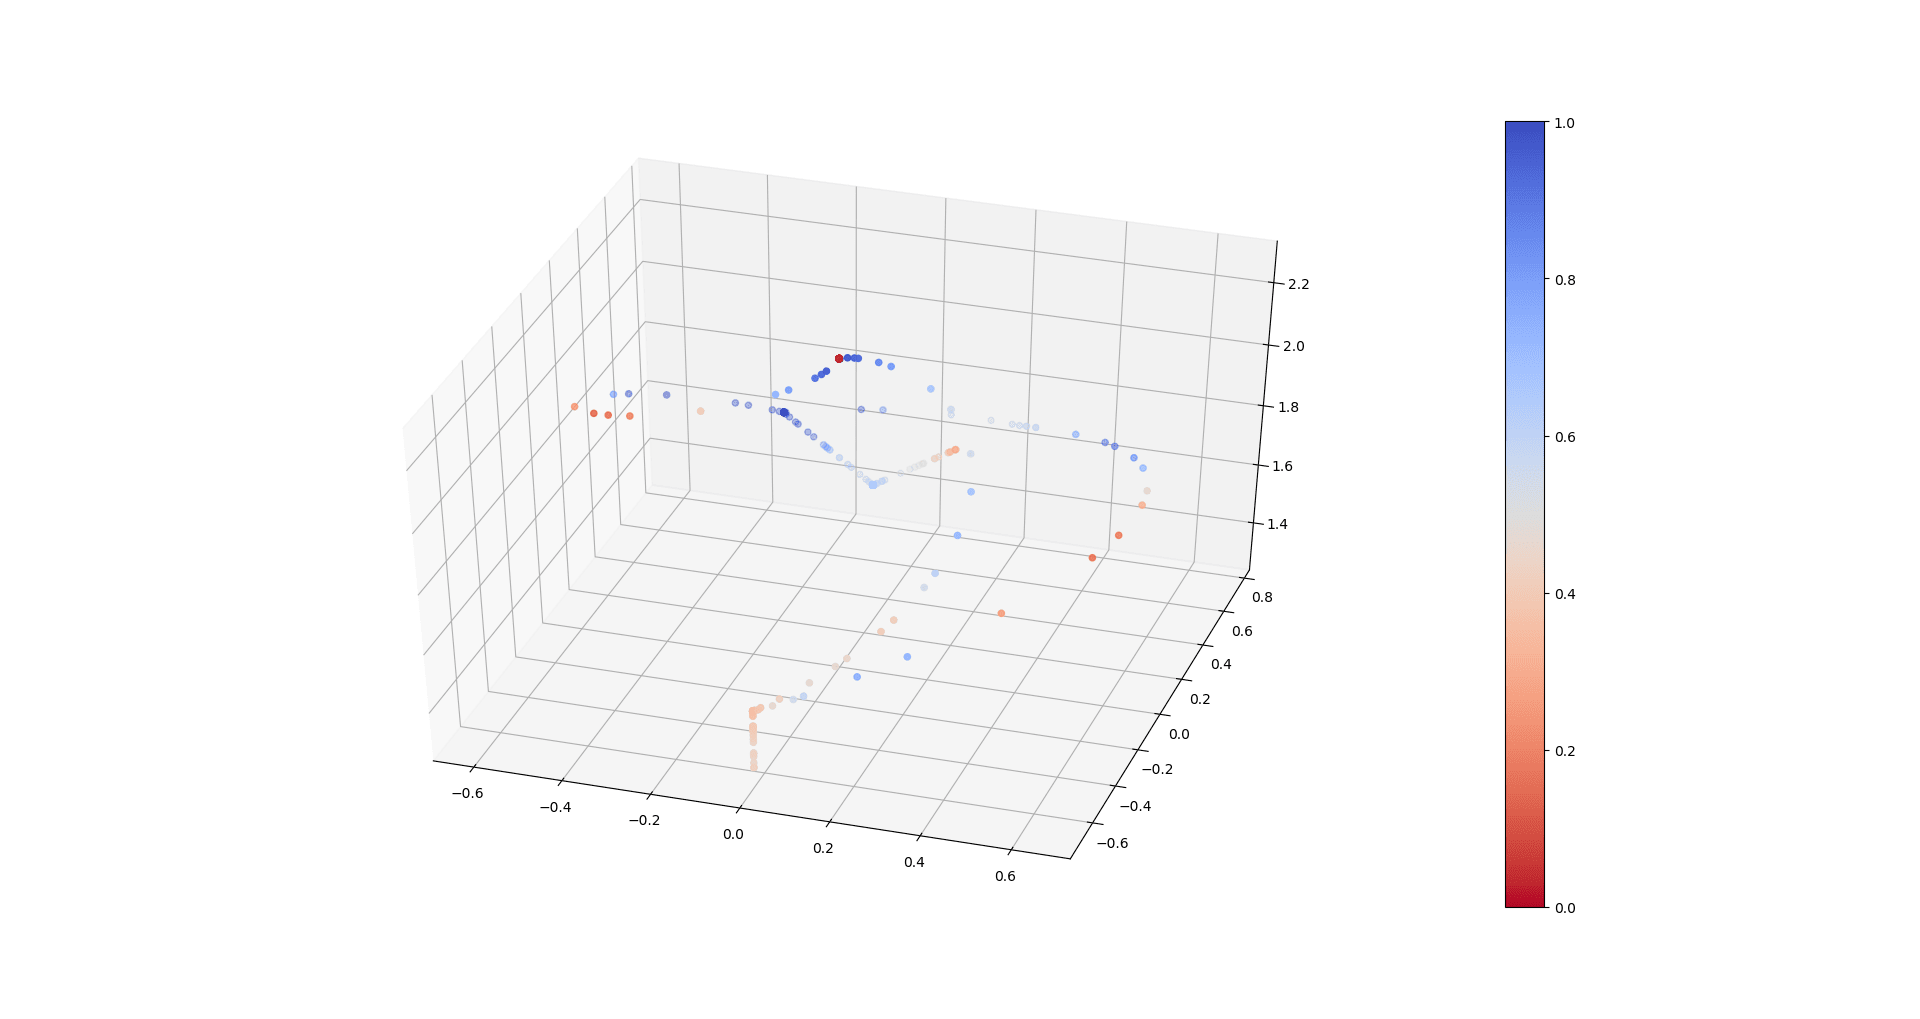
\includegraphics[width=10cm]{images/robot-planner1-manipulability-plot.png}\\
\caption{Plot the manipulability of the robot arm at sample points of the executed trajectory}
\label{robot-planner1-manipulability-plot}
\end{figure}
\end{center}

The equation \ref{joint-limit-measure} calculates a joint limit measure which is multiplied with the manipulability measure and gives the dexterity measure.
From that equation we can conclude the following:
\begin{itemize}
\item If $q_i = q_{min}$ or $q_i = q_{max}$ then the exponential is equal to 1 which means that $\mathcal{L}_{q}$ and $\mathcal{D}$ are both 0, which means 
that the robot has \textbf{no dexterity at the boundary of the task space}.
\item If the value of $q_i$ is close to it's boundary value then the dexterity approaches 0. The how much close or far it is from the boundary (or in other words 
how fast the exponential term converges) depends on the parameter $\kappa$
\item The $q_{min}, q_{max}$ are calculated from the geometry of the task-space
\end{itemize}

For maximum dexterity at most points of a trajectory in a pivoting motion, the pivot sub-
taskspace (i.e. the space of all configurations of feasible pivot motions) must be fully within 
the robot’s whole reachable taskspace, otherwise only a small range of pivot movements will be 
feasible.\\

Finding $q_{i,min}, q_{i,max}$ at \ref{joint-limit-measure} is very difficult and time-consuming especially at task spaces with more intricate geometries. 
A similar and more practical equation to \ref{joint-limit-measure} can be written for calculating the dexterity of the robot in task space:

\begin{equation}
\label{rcm-taskspace-limit-measure}
\mathcal{L}_{p}=1-e^{-\kappa (r_{max} - r)}
\end{equation}
where $r_{max}$ is the maximum radius of a circle that the tool tip can follow at a given insertion depth $z$. Moreover, at every point of the taskspace, it is $L^2 = r^2 + z^2$. 
The equation \ref{rcm-taskspace-limit-measure} however only shows dexterity in terms of approaching the boundary of the taskspace and it does not take into consideration internal points of low 
dexterity and singularities like equation \ref{dexterity-measure}.

\begin{listing}[H]
\begin{minted}[tabsize=2,breaklines,frame=lines,framesep=2mm,baselinestretch=1.2,fontsize=\footnotesize, linenos]{matlab}
x = []; y = []; z = [];
r = [];
s = 0:0.005:0.5;
L = 0.48;
k = 4.5;

for z0=-L:0.01:0
    if abs(z0)*sqrt(2) <= L
        rmax = abs(z0);
    else
        rmax = sqrt(L^2-z0^2);
    end
    for r0=0:0.02:rmax
        x = [x, r0*cos(2*pi*s)];
        y = [y, r0*sin(2*pi*s)];
        z = [z, z0*ones(size(s))];
        lp = 1-exp(-k*(rmax-r0));
        r = [r, lp*ones(size(s))];
    end
end
\end{minted}
\caption{RCM Taskpace calculation using MATLAB}
\label{code:rcm_taskspace_matlab}
\end{listing}

\begin{center}
\begin{figure}[!htb]
\centering
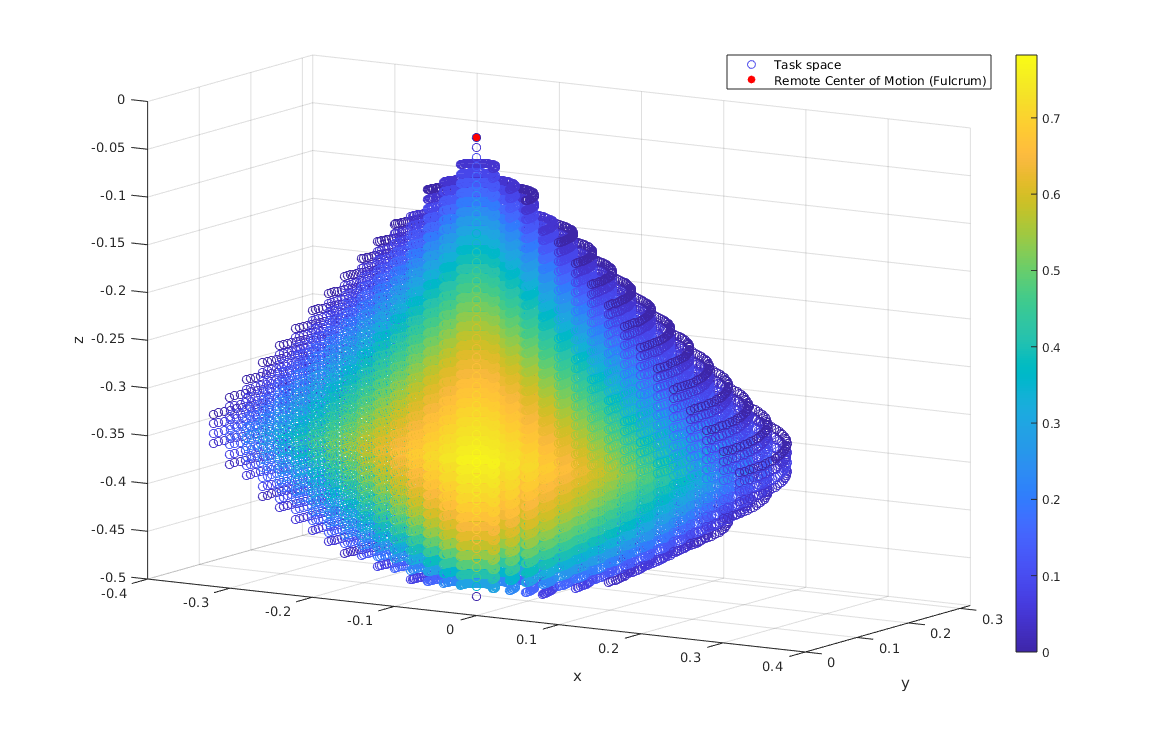
\includegraphics[width=0.8\textwidth]{images/rcm_taskspace.png}\\
\caption{Task space inside patients body. Colors with 0 or low value correspond to points with low dexterity. This is the trivial case, where no collision objects are taken into consideration}
\label{surgical-taskspace}
\end{figure}
\end{center}

All of the metrics above, measure how much reachable are various points of the surgical taskspace, but they are calculated from different perspectives, using input values from different spaces.
\begin{equation}
\mathcal{L}_{q}, \mathcal{M}: \mathbb{J} \longrightarrow \mathbb{R} \quad \textrm{and} \quad
\mathcal{L}_{p}: \mathbb{S} \longrightarrow \mathbb{R}
\end{equation}